\documentclass[conference]{IEEEtran}
\IEEEoverridecommandlockouts
% The preceding line is only needed to identify funding in the first footnote. If that is unneeded, please comment it out.
\usepackage{cite}
\usepackage{cancel}
\usepackage{amsthm}
\usepackage{amsmath,amssymb,amsfonts}
\usepackage{algorithmic}
\usepackage{graphicx}
\usepackage{textcomp}
\usepackage{url}
\usepackage{xcolor}
\def\BibTeX{{\rm B\kern-.05em{\sc i\kern-.025em b}\kern-.08em
    T\kern-.1667em\lower.7ex\hbox{E}\kern-.125emX}}
\begin{document}

\title{Métodos Numéricos para Encontrar Mínimos en Funciones Multivariables}

\author{
\IEEEauthorblockN{D. B. García Alfaro}
\IEEEauthorblockA{Universidad Centroamericana \\
00088023@uca.edu.sv}
\and
\IEEEauthorblockN{G. E. Iraheta Guardado}
\IEEEauthorblockA{Universidad Centroamericana \\
00021223@uca.edu.sv}
\and
\IEEEauthorblockN{M. A. Montes Varela}
\IEEEauthorblockA{Universidad Centroamericana \\
00042823@uca.edu.sv}
}

\maketitle

\begin{abstract}
Este trabajo presenta un análisis detallado de dos métodos numéricos fundamentales para la optimización de funciones multivariables: el descenso de gradiente y el método de Newton-Raphson multivariable. Se exploran sus fundamentos matemáticos, condiciones de estabilidad y convergencia, así como sus ventajas y limitaciones. 

A través de un ejemplo práctico de ajuste polinomial a la función seno, se ilustra la aplicación de ambos métodos, incluyendo variantes como el descenso con momento y el uso de amortiguamiento en Newton-Raphson. 

El estudio concluye con una comparación entre ambos enfoques, proporcionando criterios para seleccionar el método más adecuado según la naturaleza del problema de optimización.
\end{abstract}

\begin{IEEEkeywords}
mínimos locales, gradiente, matriz Hessiana, orden de convergencia
\end{IEEEkeywords}

\section{Introducción}
En el ámbito del Machine Learning y la optimización numérica, un problema recurrente es la minimización de funciones de costo, como el ajuste de pesos en una red neuronal para reducir el error de predicción. Este tipo de problemas suele representarse mediante funciones multivariables, donde el objetivo es encontrar parámetros que conduzcan a un mínimo local suficientemente óptimo. Dada la complejidad analítica de resolver estos problemas de manera exacta, se han desarrollado métodos numéricos iterativos, entre los que destacan el descenso de gradiente y el método de Newton-Raphson multivariable, cada uno con ventajas y limitaciones en términos de eficiencia y convergencia.

El descenso de gradiente (Gradient Descent) es un algoritmo iterativo de primer orden que ajusta los parámetros en la dirección opuesta al gradiente de la función de costo. Su simplicidad lo hace ampliamente utilizado y fácilmente escalable, incluso en problemas de alta dimensionalidad. Sin embargo, su convergencia puede ser lenta, especialmente en funciones no convexas o con variaciones abruptas en su curvatura, donde oscilaciones o estancamientos en regiones planas son comunes.

Por su parte, el método de Newton-Raphson multivariable ofrece una convergencia más rápida al utilizar información de segundo orden a través de la matriz Hessiana. No obstante, su implementación es computacionalmente costosa debido al cálculo y almacenamiento de derivadas segundas, y su eficacia depende críticamente de una inicialización cercana al óptimo, ya que en casos desfavorables puede divergir.

Este documento explora ambos métodos en profundidad: se presenta su fundamento matemático, las condiciones que garantizan estabilidad y convergencia, así como ejemplos ilustrativos de su aplicación. Finalmente, se realiza un análisis comparativo que resalta sus ventajas, desventajas y casos de uso recomendados, proporcionando así un marco de referencia para seleccionar el método más adecuado según el problema de optimización abordado.

\section{Descenso de Gradiente}\label{sec1}
\subsection{Descripción del método}\label{sec1:1}
El método de descenso del gradiente es un método para encontrar mínimos locales de una función $f$, que puede ser una función multivariable. La forma en que se encuentra el mínimo local es empezar en un punto $\omega_{0}$, evaluar $\nabla f(\omega_{0})$, y restar a $\omega_{0}$ el resultado del gradiente multiplicado por un factor $\alpha$ llamada "tasa de aprendizaje", esto para obtener el siguiente punto $\omega_{1}$. 

Extrapolando, se obtiene la siguiente expresión iterativa:
$$\omega_{k+1}=\omega _{k}-\alpha\cdot \nabla f(\omega_{k})$$
Para entender cómo funciona el método, es necesario recordar lo que es el gradiente. El gradiente de una función multivariable en un punto $\omega$, en notación matemática $\nabla f(\omega)$ es un vector cuya magnitud es la tasa de cambio máxima en $\omega$, y la dirección a la que apunta es hacia donde ocurre el mayor crecimiento en la función; y es por ello que $-\nabla f(\omega)$ es donde ocurre la tasa de mayor decrecimiento, pues es en dirección opuesta a $\nabla f(\omega)$.

Al trabajar con descenso de gradiente, evaluamos $\nabla f$ en un punto inicial $\omega_{k}$ para conocer cuál es la dirección de mayor crecimiento, y por ende, la de mayor decrecimiento, y es por eso que $\omega_{k}$ es restado un factor $\alpha$ del gradiente obtenido, para caminar un paso hacia donde la función está decreciendo; llegar a $\omega_{k+1}$, y recalcular la dirección de mayor decrecimiento en dicho punto. Así, iterativamente, se llegará a un mínimo local.

El algoritmo a seguir para el descenso de gradiente se describe por con el siguiente conjunto de pasos:
\begin{enumerate}
    \item Se inicializa el método en $k=0$ considerando un punto inicial $\omega_0$. 
    \item Calcular el gradiente de la función en el punto actual $\nabla f(\omega_k)$.
    \item Actualizar la aproximación del mínimo óptimo con la fórmula iterativa del método, considerando la tasa de aprendizaje $\alpha$ asignada $$\omega_{k+1}=\omega_{k}-\alpha \cdot \nabla f(\omega_{k})$$
    \item Verificar alguno de los criterios de convergencia $$\lvert\lvert \nabla f(\omega_{k}) \rvert\rvert < \varepsilon \quad o\quad \lvert \lvert \omega_{k+1}-\omega_{k} \rvert  \rvert <\varepsilon$$
    \item Se incrementa $k$.
\end{enumerate}
Se repiten los pasos del 2 al 5 hasta haber cumplido con un criterio de convergencia o haber alcanzado un máximo de iteraciones, retornando un $\omega_k$ como solución aproximada, es decir, como el vector de parámetros óptimo que minimiza $f(\omega)$.

\subsection{Formulación matemática}\label{sec1:2}
Supongamos una función escalar $f(\omega)$ diferenciable. Se sabe que el valor mínimo local ocurre en un punto donde la derivada de la función es igual a cero: $f'(\omega) = 0$.

Pero existen funciones demasiado complejas como para encontrar el mínimo local de forma analítica, por ello, utilizamos un método iterativo.

Lo que se pretende es minimizar la función $f(\omega)$, por lo que se deben tomar pasos en la dirección contraria a la derivada, es decir, en $-\nabla f(\omega)$. Esta idea se entiende mejor con funciones multivariables y su gradiente.

Para una función multivariable $f(\omega)$ donde $\omega \in \mathbb{R}^n$, el gradiente es $$\nabla f(\omega)=\begin{bmatrix}
\frac{ \partial f }{ \partial \omega_{0} }  \\
\frac{ \partial f }{ \partial \omega_{1} }  \\
\vdots \\
\frac{ \partial f }{ \partial \omega_{n-1} } 
\end{bmatrix}$$
Por lo que el paso de gradiente descendente se convierte en la función iterativa:
\begin{equation}
\omega_{k+1}=\omega_{k}-\alpha\cdot \nabla f(\omega_{k}) \label{grad desc}    
\end{equation}
Siendo $\alpha$ la tasa de aprendizaje que define el tamaño de los pasos en cada iteración hasta la convergencia del método en el punto $\omega$ mínimo, parando el algoritmo hasta que el gradiente es lo suficientemente cercano a cero o la diferencia entre las iteraciones presenta cambios muy pequeños, es decir, un error de aproximación menor que una tolerancia.

Como justificación geométrica, sabemos que el gradiente indica la dirección de mayor crecimiento de una función, es decir, que si se pretende minimizar la función, se debe avanzar en la dirección contraria al gradiente, en la de mayor descenso.
\subsection{Análisis de convergencia}\label{sec1:3}

El método del descenso de gradiente posee un orden de convergencia que puede variar dependiendo de las propiedades de la función $f$.

\subsubsection{Convergencia lineal}

Para este caso se asume que la función $f$ es convexa, diferenciable y satisface la condición de Lipschitz, con constante $L$, es decir:

\begin{equation}
f(y) \leq f(x) + \nabla f(x)^\top (y - x) + \frac{L}{2} \|x - y\|^2 \label{eq:lipschitz}
\end{equation}

Además, se considera un paso $\alpha$ tal que $0 < \alpha < \frac{1}{L}$, y se asume que $x^*$ es un mínimo global de $f$.

El método iterativo se define por:

\begin{equation}
x_{n+1} = x_n - \alpha \nabla f(x_n) \label{eq:iteracion}
\end{equation}

Sustituyendo $y = x_{n+1}$ y $x = x_n$ en \eqref{eq:lipschitz}:

\begin{align}
y - x &= -\alpha \nabla f(x_n) \label{eq:dy} \\
\|y - x\|^2 &= \alpha^2 \|\nabla f(x_n)\|^2 \label{eq:normdy}
\end{align}

Además, el producto escalar se evalúa como:

\begin{equation}
\nabla f(x_n)^\top (y - x) = -\alpha \|\nabla f(x_n)\|^2 \label{eq:producto}
\end{equation}

Sustituyendo \eqref{eq:dy}, \eqref{eq:normdy} y \eqref{eq:producto} en \eqref{eq:lipschitz}:

\begin{equation}
f(x_{n+1}) \leq f(x_n) - \alpha \|\nabla f(x_n)\|^2 + \frac{L \alpha^2}{2} \|\nabla f(x_n)\|^2
\end{equation}

Factorizando:

\begin{equation}
f(x_{n+1}) \leq f(x_n) - \left( \alpha - \frac{L \alpha^2}{2} \right) \|\nabla f(x_n)\|^2
\end{equation}

Dado que $\alpha \leq \frac{1}{L}$, se tiene que $\alpha - \frac{L \alpha^2}{2} \geq \frac{\alpha}{2}$, por lo que:

\begin{equation}
f(x_{n+1}) \leq f(x_n) - \frac{\alpha}{2} \|\nabla f(x_n)\|^2 \label{eq:desigualdad}
\end{equation}

Como $f$ es convexa, se cumple que:

\begin{equation}
f(x_n) - f(x^*) \leq \nabla f(x_n)^\top (x_n - x^*)
\end{equation}

Aplicando la desigualdad de Cauchy-Schwarz:

\begin{equation}
f(x_n) - f(x^*) \leq \|\nabla f(x_n)\| \cdot \|x_n - x^*\|
\end{equation}

También, bajo la hipótesis de Lipschitz para el gradiente, se tiene:

\begin{equation}
\|\nabla f(x_n)\|^2 \geq 2L (f(x_n) - f(x^*)) \label{eq:gradcotainf}
\end{equation}

Sustituyendo \eqref{eq:gradcotainf} en \eqref{eq:desigualdad}:

\begin{equation}
f(x_{n+1}) \leq f(x_n) - \alpha L (f(x_n) - f(x^*))
\end{equation}

Definiendo el error $\varepsilon_n = f(x_n) - f(x^*)$, se deduce:

\begin{equation}
\varepsilon_{n+1} \leq (1 - \alpha L)\varepsilon_n
\end{equation}

Por lo tanto, se demuestra convergencia lineal:

\begin{equation}
\boxed{\frac{|\varepsilon_{n+1}|}{|\varepsilon_n|} \leq 1 - \alpha L}
\end{equation}

\subsubsection{Convergencia sublineal}

Si $f$ no es fuertemente convexa (es decir, no posee un mínimo absoluto estrictamente definido), la rapidez de convergencia disminuye. Utilizando sumas telescópicas a partir de \eqref{eq:desigualdad}, sumando desde $n = 0$ hasta $N-1$:

\begin{equation}
\sum_{n=0}^{N-1} f(x_n) - f(x_{n+1}) \geq \frac{\alpha}{2} \sum_{n=0}^{N-1} \|\nabla f(x_n)\|^2
\end{equation}

Esta suma telescópica se reduce a:

\begin{equation}
f(x_0) - f(x_N) \geq \frac{\alpha}{2} \sum_{n=0}^{N-1} \|\nabla f(x_n)\|^2
\end{equation}

Además:

\begin{equation}
\sum_{n=0}^{N-1} \|\nabla f(x_n)\|^2 \leq \frac{2}{\alpha} (f(x_0) - f(x^*))
\end{equation}

Y como:

\begin{equation}
N \cdot \min_n \|\nabla f(x_n)\|^2 \leq \sum_{n=0}^{N-1} \|\nabla f(x_n)\|^2
\end{equation}

Se concluye:

\begin{equation}
\min_n \|\nabla f(x_n)\|^2 \leq \frac{2}{\alpha N}(f(x_0) - f(x^*)) \label{eq:min_grad}
\end{equation}

Sabemos que para funciones convexas:

\begin{equation}
f(x_n) - f(x^*) \leq \|\nabla f(x_n)\|\cdot \|x_n - x^*\| \leq R \|\nabla f(x_n)\|
\end{equation}

donde $R = \max_n \|x_n - x^*\| \leq \|x_0 - x^*\|$. Elevando ambos lados al cuadrado:

\begin{equation}
(f(x_n) - f(x^*))^2 \leq R^2 \|\nabla f(x_n)\|^2
\end{equation}

Usando \eqref{eq:min_grad}:

\begin{equation}
\min_n (f(x_n) - f(x^*))^2 \leq \frac{2R^2}{\alpha N}(f(x_0) - f(x^*))
\end{equation}

Extrayendo la raíz cuadrada:

\begin{equation}
\min_n (f(x_n) - f(x^*)) \leq \frac{R}{\sqrt{\alpha N}} \sqrt{2(f(x_0) - f(x^*))}
\end{equation}

Esto muestra una cota sublineal de convergencia, decreciendo como:

\begin{equation}
\boxed{O\left( \frac{1}{\sqrt{N}} \right)}
\end{equation}

\qed
\subsection{Condiciones de estabilidad}\label{sec1:4}
\begin{itemize}
    \item La función $f$ debe ser diferenciable en todos sus puntos, para así garantizar la obtención de un gradiente para cada punto.
    \item La función debe cumplir con la condición de Lipschitz, es decir, que la función no tenga cambios bruscos.
    \item Continuando con la condición de Lipschitz, se puede determinar una tasa de aprendizaje $\alpha \leq \frac{1}{L}$, siendo $L$ la constante de Lipschitz, para garantizar convergencia.
    \item Si $\alpha > \frac{1}{L}$, entonces no hay convergencia, pues los pasos son demasiado grandes respecto a la suavidad de la función $f$.
\end{itemize}

\subsection{Descenso con momento}\label{sec:momentum}
El Descenso de Gradiente estándar avanza en cada iteración hacia en la dirección del negativo del gradiente, que es la mayor tasa de decrecimiento, hasta llegar a un mínimo donde el gradiente es cero. Sin embargo, este enfoque se ve limitado para funciones con múltiples valles, varios de los cuales son poco profundos: Se puede converger a un mínimo, pero no es el más óptimo.

Una modificación a \eqref{grad desc} retoma una idea de la física clásica: una pelota que rueda colina abajo. Conforme avanza la pelota hacia un mínimo local, ésta acumula velocidad, lo cual le permite atravesar valles pocos pronunciados y quedar atrapada en mínimos poco óptimos, para finalmente llegar a un valle lo suficientemente convexo. Este comportamiento se modela mediante la introducción de una velocidad $v_t$ que combina la velocidad anterior con el gradiente actual.

\begin{align}
    v_{t} &= \beta v_{t-1} + (1-\beta)\nabla f(\omega_t) \label{eq:speed-calc} \\
    \omega_{t+1} &= \omega_{t} - \alpha v_{t}
    \label{eq:step-with-speed}
\end{align}

donde $v_{t}$ en \eqref{eq:speed-calc} hace referencia a la velocidad de la iteración, y se inicializa con $v_0=0$; y $\beta$ es el factor de momento, un valor dentro del intervalo $[0,1)$ que típicamente se encuentra en alrededor de 0.9. Es por medio de este mecanismo que se acelera la convergencia y se escapa de mínimos locales poco óptimos, especialmente para funciones con mucha curvatura o ruido.

\subsection{Ejemplo ilustrativo}\label{sec1:5}
Se tiene un polinomio de grado quinto \(p(x)=a_{0}+a_{1}x^{1}+a_{2}x^{2}+\dots +a_{5}x^{5}\) que quiere aproximarse a la función \(\sin(x)\) en el intervalo desde -3 a 3. El problema está en conocer cuáles son los valores que deben tomar los coeficientes \(a_{0},a_{1},a_{2},\dots,a_{5}\) para ese objetivo, por lo que se planteará una función de costo tomando como base el principio de mínimos cuadrados.
\begin{equation}
\theta(a_{0},a_{1},a_{2},\dots,a_{5})=\int_{-3}^{3} (p(x)-\sin(x))^{2}\, dx \label{eq:cost-function}
\end{equation}
La función $\theta$ representa el error cuadrático medio que hay entre la función \(\sin(x)\) y el polinomio \(p(x)\) en el intervalo $[-3,3]$; y la forma en la que se minimice el valor de la función depende del valor de los coeficientes $a_i$ de $p(x)$. Ahora, queda obtener el gradiente de la función de costo para poder realizar la iteración del descenso de gradiente.
En este caso, es posible obtener una fórmula analítica del gradiente aprovechando que $p(x)$ puede escribirse como una serie de potencias en notación sigma.
\begin{equation}
\theta(a_{0},a_{1},a_{2},\dots,a_{5})=\int_{-3}^{3}\left( \sum^{ 5 }_{ k = 0 }a_{k}x^{k} -\sin(x) \right)^{2}\, dx \label{eq:power-series-cost-function}
\end{equation}

Derivamos $\theta$ en función de los coeficientes del polinomio $p(x)$, que sería derivar $\theta$ en función de cada $a_{i}$:
\begin{equation}
\frac{ \partial \theta }{ \partial a_{i} } = \frac{ \partial  }{ \partial a_{i} } \int_{-3}^{3}\left( \sum^{ 5 }_{ k = 0 }a_{k}x^{k}-\sin(x) \right)^{2}\, dx \label{eq:partial-term}
\end{equation}
La ecuación \eqref{eq:partial-term} puede expresarse en un orden distinto, realizando la diferenciación antes de la integración, haciendo uso del teorema de Leibniz para diferencia integrales con parámetros. Por lo tanto, se tiene que la derivada de $\theta$ respecto a un parámetro $a_i$ es:
\begin{equation}
\int_{-3}^{3}\frac{ \partial  }{ \partial a_{i} } \left( \sum^{ 5 }_{ k = 0 }a_{k}x^{k}-\sin(x) \right)^{2}\, dx \label{eq:flipped-partial-term}
\end{equation}
De esta forma, se obtiene la derivada parcial de $\theta$ respecto a cualquiera de sus parámetros $a_i$.
\begin{equation}
\frac{ \partial \theta }{ \partial a_{j} } = 2\int_{-3}^{3} x^{j}\,  (p(x)-\sin(x))\, dx \label{term:grad-component}
\end{equation}
El gradiente de la función de costo, que es el gradiente a utilizar para \ref{grad desc} iterativamente, tiene la forma:
\begin{equation}
\nabla\theta=2\begin{bmatrix}
\int_{-3}^{3} x^{0}\, (p(x)-\sin(x)) \, dx  \\
\int_{-3}^{3} x^{1}\, (p(x)-\sin(x)) \, dx  \\
\int_{-3}^{3} x^{2}\, (p(x)-\sin(x)) \, dx \\
\vdots \\
\int_{-3}^{3} x^{5}\, (p(x)-\sin(x)) \, dx
\end{bmatrix} \label{gradient}
\end{equation}

\subsubsection{Método estándar}\label{sec:standard-example}
Se optó por utilizar una tasa de aprendizaje de $\alpha=1\times10^{-5}$, además de utilizar métodos numéricos para obtener los resultados de las integrales que componen al gradiente. Después de mil iteraciones, se alcanzó un mínimo local donde los coeficientes $a_i$ no cambiaban mucho, dejando como resultado una aproximación de $\sin(x)$ que minimizó el error cuadrático. La comparación del $p(x)$ con la función $\sin(x)$ se aprecia en Fig. \ref{gradient-plot}. Se partió de un arreglo de coeficientes aleatorio.

\begin{figure}[htbp]
\centerline{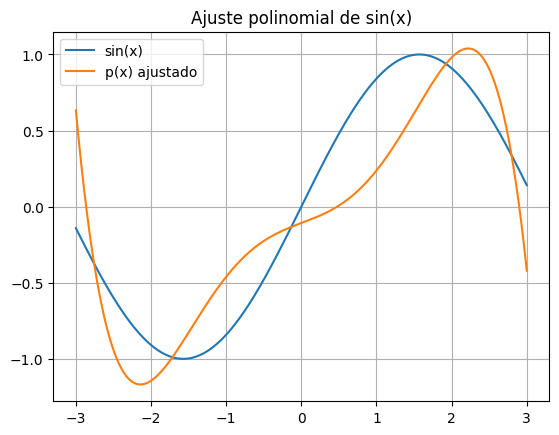
\includegraphics[width=0.45\textwidth]{fig1.png}}
\caption{Ajuste polinomial de $sin(x)$}
\label{gradient-plot}
\end{figure}

En la Fig. \ref{gradient-error} se observa el error cuadrático medio en cada iteración, evaluando la función de costo por cada arreglo de valores. Se puede apreciar una forma racional en el decrecimiento del error.

\begin{figure}[htbp]
\centerline{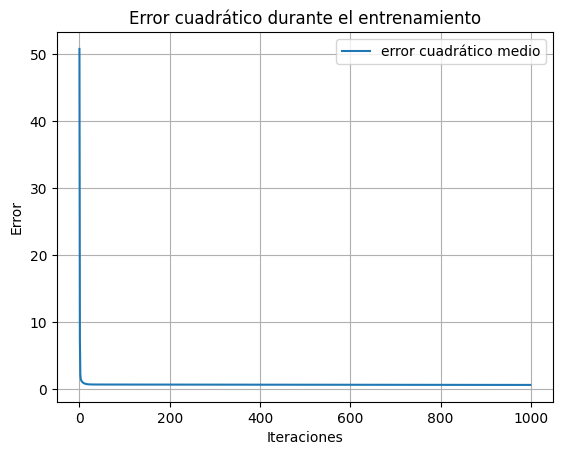
\includegraphics[width=0.45 \textwidth]{fig2.png}}
\caption{Evolución del error cuadrático medio}
\label{gradient-error}
\end{figure}

La aproximación del polinomio obtenido usando iteración de descenso de gradiente se muestra a continuación:
\begin{multline*}
    p(x)=-0.099445+0.197967x+0.001409x^{2} \\
    +0.175170x^{3}+0.002015x^{4}-0.023861x^{5}
\end{multline*}

\subsubsection{Método con momento}\label{sec:momentum-example}
Observando que la aproximación del método no es óptima, se puede utilizar la modificación con momento mencionada en la sección \ref{sec:momentum} para poder llegar a una mejor aproximación. Una consecuencia de este método es que la tasa de aprendizaje cambia, el valor establecido en \ref{sec:standard-example} ahora no permite convergencia al ser muy pequeño; y ahora se estableció $\alpha=1\times10^{-3}$ y un factor de momento $\beta=0.995$. Fig. \ref{momentum-plot} muestra la aproximación de $p(x)$ después de mil iteraciones, comparando con el resultado de la sección \ref{sec:standard-example}.

\begin{figure}[htbp]
\centerline{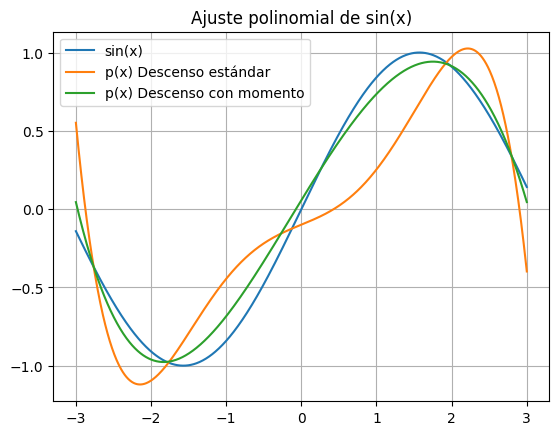
\includegraphics[width=0.45 \textwidth]{fig5.png}}
\caption{Ajuste polinomial de $\sin(x)$}
\label{momentum-plot}
\end{figure}

En Fig. \ref{momentum-error}, la gráfica muestra cómo el error cuadrático medio disminuye y aumenta, una visualización de los mínimos poco pronunciados por los que se pasó para luego converger en un mínimo más óptimo.

\begin{figure}[htbp]
\centerline{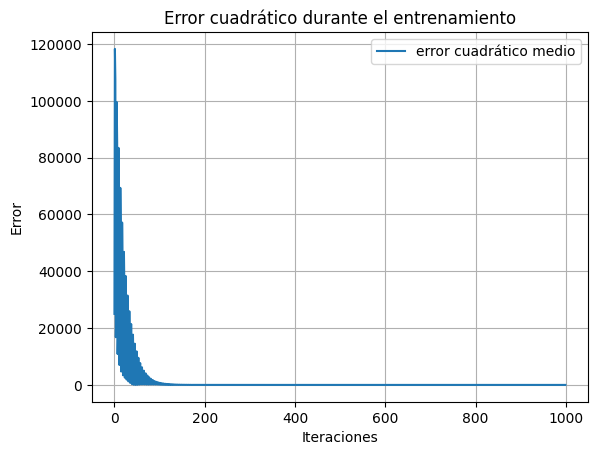
\includegraphics[width=0.45 \textwidth]{fig6.png}}
\caption{Evolución del con Descenso de Gradiente con momento}
\label{momentum-error}
\end{figure}

El polinomio aproximado resultante con descenso con momento es el siguiente:
\begin{multline*}
    p(x)=0.056855+0.783697x-0.035206x^{2} \\
    -0.072163x^{3}+0.003762^{4}-0.001656x^{5}
\end{multline*}

\subsection{Ventajas y desventajas del método}\label{sec1:6}
\subsubsection{Ventajas}
\begin{itemize}
    \item El método de descenso del gradiente es escalable a muchos parámetros, dado que funciona correctamente con un gran número de parámetros. Por ello, es ampliamente utilizado en Machine Learning, por ejemplo. Es eficiente para conjuntos de datos grandes.
    \item Es un método fácil de implementar con una lógica relativamente sencilla.
    \item Es generalizable, puede ser aplicado a varias funciones de costo.
\end{itemize}
\subsubsection{Desventajas}
\begin{itemize}
    \item Es demasiado sensible a la tasa de aprendizaje $\alpha$: si es muy grande puede divergir; si es muy pequeña, puede converger muy lentamente o no alcanzar el mínimo local.
    \item Puede atascarse en mínimos locales o puntos de silla en funciones no convexas. Se requiere de variaciones para lograr escapar de regiones no óptimas.
    \item Requiere que la función de costo sea diferenciable respecto a todos los parámetros.
\end{itemize}

\section{Newton-Raphson multivariable}

\subsection{Descripción del método}
El método de Newton-Raphson es una técnica iterativa usada para encontrar los puntos críticos de una función escalar o vectorial de múltiples variables, hablando específicamente de optimización, se utiliza para encontrar los mínimos locales de una función suave. Utiliza información de segundo orden, es decir, toma en cuenta la curvatura de la función para construir una aproximación cuadrática de la función y determinar cómo avanzar hacia el mínimo.

La estrategia que implementa el método de Newton consiste en modelar localmente la función que se desea minimizar con una parábola multidimensional. Dicha parábola se construye a partir del punto actual usando la expansión de Taylor en segundo orden. Posteriormente, se calcula el mínimo de la parábola y el punto obtenido se usa como la siguiente aproximación del mínimo.
El método busca resolver el sistema de ecuaciones:

$$\nabla f(\omega)=0$$

Lo anterior indica, que se pretende encontrar los puntos en donde la pendiente de la recta tangente a la curva es nula, sabiendo que entre estos puntos podemos encontrar los mínimos locales si la curvatura es \textbf{positiva}.

Por ello, Newton utiliza la matriz Hessiana, verificando que sea positiva y definida para asegurar que las aproximaciones se están acercando al mínimo de la función y no hacia otro punto crítico como un máximo o punto de silla. La fórmula iterativa que implementa el método de Newton es
\begin{equation}
    \omega_{k+1}=\omega_k-H_f(\omega_k)^{-1}\cdot\nabla f(\omega_k) \label{eq:newton-raphson}
\end{equation}

Dada la fórmula y un punto inicial $\omega_0$, el algoritmo de Newton para minimización realiza los siguientes pasos:

\begin{enumerate}
    \item Primeramente evalúa el gradiente de la función $\nabla f(\omega_k)$ en el punto actual $\omega_k$, indicando la dirección de mayor pendiente.
    \item Luego evalúa la matriz Hessiana $H_f(\omega_k)$, que representa la curvatura, es decir, como cambia el gradiente.
    \item Construye una aproximación cuadrática local de la función en torno al punto actual $\omega_k$ usando Taylor.
    \item Encuentra el mínimo de la función cuadrática aproximada, derivando dicha parábola.
    \item Se actualiza el punto a una nueva estimación más cercana al punto real con la fórmula iterativa 
    \begin{equation}
        \omega_{k+1}=\omega_k+\Delta \omega_k
    \end{equation}
    
    Donde $\Delta\omega_k=-H_f(\omega_k)\cdot\nabla f(\omega_k)$.
\end{enumerate}

El procedimiento anterior se repite iterativamente con el objetivo de acercarse progresivamente al mínimo local de la función. Sin embargo, dado que no se puede iterar indefinidamente en la práctica, es necesario establecer criterios de paro.

\subsubsection{Criterios de paro}
Todos los criterios de paro se basan en verificar que cierto valor se encuentre por debajo de una tolerancia epsilónica $\epsilon$:
\begin{itemize}
    \item El gradiente: $$\Vert \nabla f(\omega_{k})\Vert <\epsilon$$
    \item Error absoluto: $$\Vert \omega_{k+1}-\omega_{k}\Vert < \epsilon$$
    \item Error absoluto de las imágenes: $$\vert f(\omega_{k+1})-f(\omega_{k})\vert$$
    \item Número máximo de iteraciones:$$k=k_{max}$$
\end{itemize}

El método de Newton se vuelve bastante bueno en términos de eficiencia dado que al considerar la curvatura el método puede ajustar el tamaño del paso de forma automática y adaptativa sin depender de una tasa de aprendizaje fija, puede corregir la dirección incluso si el gradiente previamente apunta a una zona menos eficiente, y puede converger en menos iteraciones que métodos de primer orden como Descenso de Gradiente. Esto se debe a que el método cerca de la solución tiene una convergencia \textbf{cuadrática}, indicando que el número de cifras correctas se duplica por cada nueva estimación en cada iteración.

\subsection{Formulación matemática}
Se tiene una función \( f:\mathbb{R}^n\to\mathbb{R} \) de la cual buscamos encontrar el mínimo local, es decir, se busca un punto \( \omega^*\in\mathbb{R}^n \) tal que
\begin{equation}
f(\omega^{*})\leq f(\omega),\quad \text{para valores cercanos a } \omega^{*}
\label{eq:minimo_local}
\end{equation}

Para minimizar \( f(\omega) \) buscamos los puntos críticos donde el gradiente se anula, por lo que minimizar la función es equivalente a resolver el sistema de ecuaciones no lineal:
\begin{equation}
\nabla f(\omega)=0
\label{eq:gradiente_cero}
\end{equation}

Se aplica el método de Newton-Raphson para resolver el sistema de ecuaciones. Sea \( f(\omega) \) dos veces continuamente diferenciable, expandimos en serie de Taylor alrededor del punto actual \( \omega_k \):
\begin{multline}
f(\omega)\approx f(\omega_k)+\nabla f(\omega_k)^T(\omega-\omega_k)+ \\
\frac{1}{2}(\omega-\omega_k)^T H_f(\omega_k)(\omega-\omega_k)
\label{eq:taylor_segundo_orden}
\end{multline}

Ahora, para minimizar la aproximación encontrada por medio de la expansión de Taylor de segundo orden, derivamos respecto de \( \omega \) y se iguala a cero:
\begin{equation}
\nabla f(\omega_k)+H_f(\omega_k)(\omega_{k+1}-\omega_k)=0
\label{eq:gradiente_aproximado}
\end{equation}

Despejando \( \omega_{k+1} \) para encontrar una nueva aproximación del mínimo de la función:
\begin{equation}
\omega_{k+1}=\omega_k-H_f(\omega_k)^{-1}\cdot\nabla f(\omega_k)
\label{eq:newton_actualizacion}
\end{equation}

\subsection{Análisis de convergencia}
Para poder demostrar el orden de convergencia del método de Newton-Raphson en optimización, tenemos que mantener las hipótesis necesarias:
\begin{itemize}
  \item La función $f$ debe ser tres veces continua diferenciable, es decir, sus derivadas parciales tienen primera, segunda y terceras derivadas continuas.
  \item Su gradiente evaluado en el punto final debe ser $0$, es decir, $\nabla f(\omega^{*})=0$.
  \item La matriz Hessiana debe ser definida positiva, es decir, que $\mathbf{x}^{T}H_{f}\mathbf{x}>0$ para todo vector no nulo $\mathbf{x}\in \mathbb{R}^{n}$.
  \item $\omega_{k}$ debe de ser lo más cercano posible a $\omega^{*}$.
\end{itemize}

Sea $E_{k}=\omega_{k}-\omega^{*}$. La expansión de Taylor del gradiente centrada en $\omega^{*}$ está dada por:

\begin{equation}
\nabla f(\omega_{k})=\nabla f(\omega^{*})+\nabla^{2}f(\omega^{*})(\omega_{k}-\omega^{*})+R_{1}
\end{equation}

Donde:
\begin{itemize}
  \item $\nabla f(\omega^{*})=0$ por la definición del punto mínimo.
  \item $R_{1}$ es término cúbico del error: $R_{1}=\frac{1}{2}\nabla f(\xi)(\omega_{k}-\omega^{*})^{2}$
\end{itemize}

Por lo que:

\begin{equation} \label{taylor_polinomial}
\nabla f(\omega_{k})=\nabla^{2}f(\omega^{*})E_{k}+\mathcal{O}(\Vert E_{k}\Vert ^{2})
\end{equation}

A su vez, se puede realizar la expansión de la Hessiana en Taylor:

\begin{equation}
\nabla^{2}f(\omega_{k})=\nabla^{2} f(\omega^{*})+R_{1}
\end{equation}

Ya que $R_{1}=\nabla f(\xi)(\omega_{k}-\omega^{*})$, entonces:

\begin{equation} \label{O_notation}
\nabla^{2}f(\omega_{k})=\nabla^{2} f(\omega^{*})+\mathcal{O}(\Vert E_{k} \Vert)
\end{equation}

Recordando la iteración del método:

\begin{equation}
\omega_{k+1}=\omega_{k}-[H_{f}(\omega_{k})]^{-1}\nabla f(\omega_{k})
\end{equation}

Buscando encontrar el error $E_{k+1}$:

\begin{equation} \label{error_with_grad}
E_{k+1}=\omega_{k+1}-\omega^{*}=\omega_{k}-\omega^{*}-[H_{f}(\omega_{k})]^{-1}\nabla f(\omega_{k})
\end{equation}

Reemplazando \eqref{taylor_polinomial} en \eqref{error_with_grad}:

\begin{equation}
E_{k+1}=\omega_{k}-\omega^{*}-[H_{f}(\omega_{k})]^{-1}(\nabla^{2}f(\omega^{*})E_{k}+\mathcal{O}(\Vert E_{k} \Vert^{2}))
\end{equation}

Por fórmula de la inversión de matrices perturbadas y la evaluación de \eqref{O_notation}:

\begin{equation}
[H_{f}(\omega_{k})]^{-1}=[\nabla^{2}f(\omega_{k})]^{-1}=[\nabla^{2}f(\omega_{k})]^{-1}+\mathcal{O}(\Vert E_{k}\Vert )
\end{equation}

Sustituyendo en la ecuación anterior:

\begin{multline*}
    E_{k+1}=E_{k}-([\nabla^{2}f(\omega_{k})]^{-1}+\\
    \mathcal{O}(\Vert E_{k} \Vert))(\nabla^{2}f(\omega^{*})E_{k}+\mathcal{O}(\Vert E_{k} \Vert^{2}))
\end{multline*}

Expandiendo:
\begin{equation}
    \begin{array}{cl}
        E_{k+1} &= E_k - (
            \cancelto{1}{[\nabla^2 f(\omega_k)]^{-1} \cdot \nabla^2 f(\omega_k)} E_k \\
        & + \cancelto{\mathcal{O}(\Vert E_k \Vert^2)}{[\nabla^2 f(\omega_k)]^{-1} \cdot \mathcal{O}(\Vert E_k \Vert)} \\
        & +\cancelto{\mathcal{O}(\Vert E_k \Vert^2)}{\mathcal{O}(\Vert E_k \Vert) \cdot \nabla^2 f(\omega_k)} \\
        & + \cancelto{\mathcal{O}(\Vert E_k \Vert^3)}{\mathcal{O}(\Vert E_k \Vert) \cdot \mathcal{O}(\Vert E_k \Vert^2)})
    \end{array}
\end{equation}

Quedando:

\begin{equation}
    E_{k+1} =\mathcal{O}(\Vert E_{k}\Vert ^{2})+\mathcal{O}(\Vert E_{k}\Vert ^{3})
\end{equation}

Debido a que se toma el orden más bajo, entonces obtenemos que:

\begin{equation}
E_{k+1}=\mathcal{O}(\Vert E_{k}\Vert ^{2})
\end{equation}

Demostrando así, que el método de Newton-Raphson multivariable de optimización converge cuadráticamente.

\subsection{Condiciones de estabilidad}

\begin{enumerate}
    \item La función objetivo $f(\omega)$ debe ser suave y continuamente diferenciable hasta segundo orden garantizando que tanto el gradiente $\nabla f(\omega)$ como la Hessiana $H_f(\omega)$ existen y son continuas, lo cual resulta necesario para la validez de la aproximación cuadrática por la serie de Taylor de segundo orden.

    \item Si el punto mínimo es $\omega^*$, entonces la matriz Hessiana en dicho punto debe ser positiva definida, es decir, la función tiene curvatura positiva en todas las direcciones, el punto crítico es un mínimo local estricto, asegurando no converger en máximos ni puntos de silla y la dirección de Newton es un descenso verdadero. 
    Esto se puede demostrar verificando los autovalores no nulos de la matriz Hessiana, que todos ellos sean positivos. Si la matriz Hessiana no cumple esta condición, el método puede converger diverge.

    \item Newton no es globalmente convergente por sí mismo, requiere que el punto inicial $\omega_0$ se encuentre lo suficientemente cerca del mínimo local verdadero, esto con el fin de garantizar la convergencia del método y la convergencia cuadrática eficiente.
    Si el punto inicial se encuentra lejos del mínimo, el método puede divergir o converger a otro punto crítico.

    \item La Hessiana debe ser invertible, dado que en cada iteración se necesitar resolver el sistema de ecuaciones
    $$H_{f}(\omega_{k})\cdot\Delta\omega_{k}=-\nabla f(\omega_{k})$$
    Por lo tanto, la matriz Hessiana debe cumplir con que su determinante sea diferente de cero para que exista su inversa y el sistema posea una solución única.
\end{enumerate}

\subsection{Amortiguamiento del paso}\label{sec:damped-method}
El método de Newton-Raphson requiere de que el punto inicial no se encuentre lejos del mínimo para converger; sin embargo en funciones cuya forma no es conocida, especialmente para funciones $\mathbb{R}^{n}\to\mathbb{R}$, se vuelve muy complicado empezar desde una región cercana a un mínimo; y si la matriz Hessiana es inestable, la divergencia y convergencia es determinada por centésimas en el punto inicial. Entonces, para permitir convergencia, se utiliza un factor de amortiguamiento $\eta$ en el método.

La fórmula iterativa modificada con amortiguamiento utilizada es la siguiente:

\begin{equation}
    \omega_{k+1}=\omega_{k}-\eta H_{f}(\omega_{k})\cdot\nabla f(\omega_{k})
    \label{eq:damped-newton-raphson}
\end{equation}

donde $\eta$ es el parámetro de amortiguamiento, típicamente un valor en el intervalo $(0,1]$. Este factor regula la magnitud del paso en cada iteración mientras conserva la dirección en la que el método desea converger; y se usa en caso de que el método de Newton-Raphson original no converja.

\subsection{Ejemplo ilustrativo}\label{sec:example-newton-raphson}
Tendremos el mismo ejemplo hecho en la sección \ref{sec1:5} para probar el Descenso de Gradiente: Encontrar los coeficientes $a_0, a_1, \dots, a_5$ que mejor aproximan un polinomio $p(x)$ de quinto grado a la función $\sin(x)$ en el intervalo $x\in[-3,3]$. Para ello se planteó la función de costo \eqref{eq:cost-function} haciendo uso de mínimos cuadrados; y además se obtuvo \eqref{gradient}, el término del gradiente de la función de costo.

Sin embargo, la fórmula iterativa para el método de Newton-Raphson multivariable requiere de la matriz Hessiana de la función de costo. Pero, gracias al gradiente, tenemos un término general para la primera derivada parcial de una constante $a_i$, así que podemos obtener un término general para las segundas derivadas $a_j$.

Por medio de \eqref{term:grad-component} se tiene el término general para las componentes del gradiente
$$
\frac{ \partial \theta }{ \partial a_{i} } =2\int_{-3}^{3} x^{i}(p(x)-\sin(x))\, dx
$$
Dado que la matriz Hessiana deriva la primera derivada parcial con respecto a todas las variables por segunda vez, solo queda calcular esta nueva expresión:
\begin{equation}
    \frac{ \partial  }{ \partial a_{j} } \frac{ \partial \theta }{ \partial a_{i} } =\frac{\partial^{2} \theta}{\partial a_{i} \partial a_{j}}=\frac{ \partial }{ \partial a_{j} } 2\int_{-3}^{3} x^{i}(p(x)-\sin(x))\, dx
    \label{eq:second-partial-derivative}
\end{equation}

Nuevamente, utilizando el Teorema de Leibniz, transformamos \eqref{eq:second-partial-derivative}:

\begin{equation}
    \frac{\partial^{2} \theta}{\partial a_{i} \partial a_{j}}=2\int_{-3}^{3}\left[ \frac{ \partial }{ \partial a_{j} } x^{i}(p(x)-\sin(x)) \right]\, dx =2\int_{-3}^{3}x^{i}x^{j}\, dx 
\end{equation}
Entonces, los términos de la matriz Hessiana son descritos por el siguiente término general:
\begin{equation}
    H_{ij}=2\int_{-3}^{3} x^{i+j} \, dx \label{term:hessian-item}
\end{equation}

Evaluar para los coeficientes desde $a_{0}$ hasta $a_{5}$ devuelve la siguiente matriz Hessiana:

\begin{equation}
    H=
    \begin{bmatrix}
        12 & 0 & 36 & 0 & \frac{972}{5} & 0 \\
        0 & 36 & 0 & \frac{972}{5} & 0 & \frac{8748}{7} \\
        36 & 0 & \frac{972}{5} & 0 & \frac{8748}{7} & 0 \\
        0 & \frac{972}{5} & 0 & \frac{8748}{7} & 0 & 8748 \\
        \frac{972}{5} & 0 & \frac{8748}{7} & 0 & 8748 & 0 \\
        0 & \frac{8748}{7} & 0 & 8748 & 0 & \frac{708588}{11}
    \end{bmatrix}
    \label{mat:hessian}
\end{equation}

Dado que \eqref{eq:newton-raphson} requiere de la inversa de la matriz Hessiana, se tiene que encontrar la inversa de \eqref{mat:hessian}
\begin{align}
        \begin{bmatrix}
            \frac{75}{256} & 0 & -\frac{175}{1152} & 0 & \frac{35}{2304} & 0 \\
            0 & \frac{1225}{2304} & 0 & -\frac{245}{1152} & 0 & \frac{385}{20736} \\
            -\frac{175}{1152} & 0 & \frac{245}{1728} & 0 & -\frac{175}{10368} & 0 \\
            0 & -\frac{245}{1152} & 0 & \frac{175}{1728} & 0 & -\frac{2695}{279936} \\
            \frac{35}{2304} & 0 & -\frac{175}{10368} & 0 & \frac{1225}{559872} & 0 \\
            0 & \frac{358}{20736} & 0 & -\frac{2695}{279936} & 0 & \frac{539}{559872}
        \end{bmatrix}
    \label{mat:inv-hessian}
\end{align}

Para este caso, se tuvo la suerte de que \eqref{mat:hessian} resultó ser una matriz constante. De no serlo, tendría que evaluarse para cada término el vector $\omega_{k}$ por cada iteración en \eqref{mat:inv-hessian}, lo cual puede ser muy costoso computacionalmente. Sin embargo, ahora hay que multiplicar $H^{-1}\cdot\nabla\theta(\omega_{k})$ por cada iteración, una operación costosa, pues es una multiplicación entre matrices.

Ya se tienen todos los elementos necesarios para poder realizar la iteración de Newton-Raphson, partiendo con las valores aleatorios para las contantes $a_i$. No obstante, el método no converge ya que \eqref{eq:newton-raphson} produce saltos demasiado grandes para este caso, probablemente porque el punto inicial no se encuentra tan cerca de un mínimo local como se esperaba. Es por ello que, para permitir convergencia, se utilizó la fórmula con amortiguamiento \eqref{eq:damped-newton-raphson}.

Para reducir la inestabilidad del método, se encontró una factor de amortiguamiento $\eta=0.04$, sin embargo se requirieron varios intentos para obtener un mínimo local satisfactorio. No obstante, por medio de este método se logró obtener un resultado más óptimo con menos iteraciones (300 iteraciones) que con Descenso de Gradiente; cómo se puede observar en Fig. \ref{newton-raphson-plot}.

\begin{figure}[htbp]
\centerline{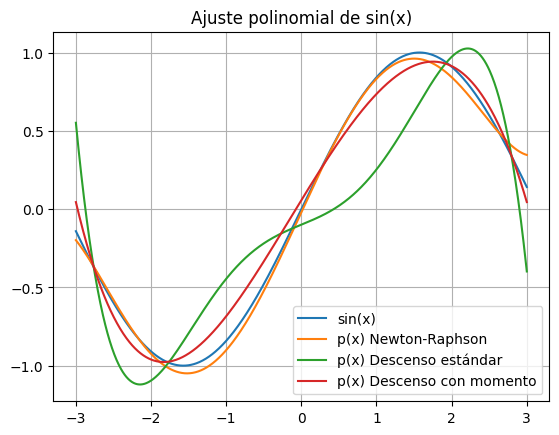
\includegraphics[width=0.45\textwidth]{fig3.png}}
\caption{Ajuste polinomial de $sin(x)$ con Newton-Raphson}
\label{newton-raphson-plot}
\end{figure}

El error cuadrático medio también disminuye converge mucho más rápido a cero debido a que el método de Newton-Raphson multivariable tiene una rapidez de convergencia cuadrática. La minimización del error se puede observar en Fig. \ref{newton-raphson-error}. El error cuadrático medio también se minimizó lo más que pudo con el Descenso de Gradiente como también muestra Fig. \ref{error_with_grad} en pocas iteraciones, pero el mínimo local alcanzado con Newton-Raphson multivariable se aproxima con menor error.

\begin{figure}[htbp]
\centerline{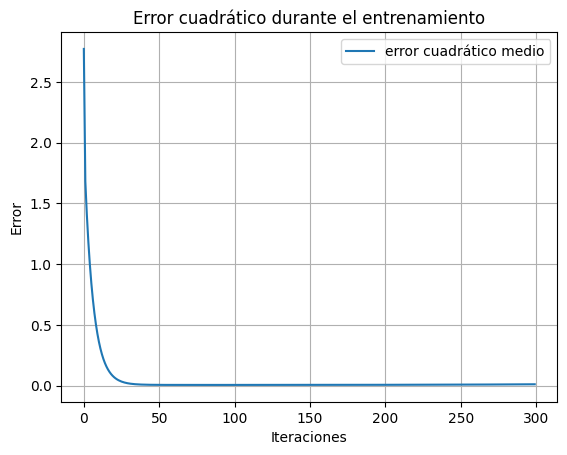
\includegraphics[width=0.45\textwidth]{fig4.png}}
\caption{Evolución del error cuadrático medio usando Newton-Raphson}
\label{newton-raphson-error}
\end{figure}

La aproximación del polinomio obtenido usando iteración de descenso de gradiente se muestra a continuación:

\begin{multline*}
    p(x) = -0.019534+1.043933x-0.017897x^{2} \\
    -0.186261x^{3}+0.003139x^{4}+0.008928x^{5}
\end{multline*}

\subsection{Ventajas y desventajas}

\subsubsection{Ventajas}
\begin{itemize}
    \item El método de Newton-Raphson tiene convergencia cuadrática si se cumplen las condiciones de estabilidad, por lo cual converge muy rápidamente. La cantidad de cifras correctas y precisión se duplican por cada iteración del método.  
    \item Dado que considera la curvatura de la función mediante la matriz Hessiana, no solo el gradiente, se producen pasos más eficientes en cuánto a precisión de búsqueda.
    \item El método puro no requiere de una tasa de aprendizaje fija, a diferencial del Descenso de Gradiente; esto dado que se ajusta manualmente adaptándose en cada iteración usando a la matriz Hessiana.
    \item Al utilizar una expansión por serie de Taylor de segundo orden, se modela mejor el comportamiento real de las funciones no lineales.
\end{itemize}

\subsubsection{Desventajas}
\begin{itemize}
    \item Dado que necesita calcular la matriz Hessiana, computacionalmente puede resultar seriamente costoso y calcular las segundas derivadas analíticamente puede ser complicado o hasta imposible.
    \item El método puede converger a puntos que no son mínimos dado que busca puntos críticos en donde el gradiente de la función es cero, puede converger a máximos o puntos de silla, no necesariamente a mínimos. Por ello, la condición que dicta que la Hessiana debe ser positiva definida se debe cumplir, para asegurar la convergencia del método en un mínimo.
    \item Si el punto inicial está muy lejos del mínimo local el método puede divergir, necesita una buena estimación inicial; o bien utilizar un factor de amortiguamiento para asegurar estabilidad, cumpliendo un rol similar a la de la tasa de aprendizaje del Descenso de Gradiente.
    \item El método no es apto para funciones ruidosas o no suaves, requiere funciones continuas y dos veces diferenciables.
\end{itemize}

\section{Análisis comparativo de los métodos}
Los métodos de Descenso de Gradiente y Newton-Raphson multivariable son herramientas eficaces para la localización de mínimos en funciones multivariables. Cada uno presenta ventajas, limitaciones y contextos de aplicación específicos que los hacen más adecuados según el tipo de problema abordado.

\begin{table}[htbp]
\caption{Comparación de los Métodos}
    \begin{center}
        \begin{tabular}{|p{3.5cm}|p{3.5cm}|}
        \hline
        \textbf{Descenso de Gradiente} & \textbf{Método de Newton-Raphson} \\
        \hline
        Método de primer orden, solo usa gradiente &
        Método de segundo orden, usa gradiente y matriz Hessiana \\
        \hline
        Velocidad de convergencia lineal o sublineal & Velocidad de convergencia cuadrática si se cumplen condiciones de estabilidad \\
        \hline
        Solo utiliza primeras derivadas, gradiente & Se requiere de segundas derivadas para la matriz Hessiana \\
        \hline
        Bajo costo computacional & Alto costo computacional al calcular la inversa de la matriz Hessiana por cada iteración \\
        \hline
        Moderadamente sensible al punto inicial & Altamente sensible, requiere de estar cerca de un mínimo para que haya convergencia. \\
        \hline
        La estabilidad depende críticamente de la elección de la tasa de aprendizaje $\alpha$ & Depende de la positividad y estabilidad de la matriz Hessiana \\
        \hline
        Puede atascarse en mínimos no óptimos o puntos de silla & Puede converger a puntos de silla o máximos si la Hessiana no cumple con los criterios de estabilidad \\
        \hline
        Fácil de implementar, escalable para funciones complejas & Un poco más difícil de implementar, y por la matriz Hessiana, no es fácil escalarla para lidiar con funciones de varias variables \\
        \hline
        \end{tabular}
    \label{tab:comparison}
    \end{center}
\end{table}

Utilizando como base los ejemplos ilustrativos de las secciones \ref{sec1:5} y \ref{sec:example-newton-raphson}, se observó que el método de descenso de gradiente estándar tiene problemas para converger en un mínimo óptimo; e incluso cuando lo logra, requiere un número considerable de iteraciones para alcanzar una solución aceptable. No obstante, su implementación es sencilla; y los problemas con los mínimos locales pueden solucionarse con variantes del método, como es el caso del Descenso con Momento mencionado en la sección \ref{sec:momentum}.

Comparado con el Newton-Raphson multivariable, Descenso de Gradiente no es tan preciso y toma muchas más iteraciones iteraciones alcanzar algo que con el método de Newton solo tomó 300 iteraciones. No obstante, esto solo se pudo tras utilizar el método amortiguado discutido en la sección \ref{sec:damped-method}, ya que el método estándar era muy inestable, y es difícil establecer un punto inicial cerca de un mínimo sin saber cómo se ve la función, especialmente cuando \eqref{eq:cost-function} es una función $\mathbb{R}^{6}\to\mathbb{R}$. En nuestro ejemplo, el tiempo de ejecución fue menor con Newton, lo cual podría atribuirse a que, en este caso particular, la matriz Hessiana fue constante, simplificando los cálculos.

\section{Conclusión}
A lo largo de este documento se ha demostrado que tanto el descenso de gradiente como el método de Newton-Raphson multivariable son herramientas poderosas para la optimización de funciones multivariables, cada uno con sus propias fortalezas y debilidades. 

El descenso de gradiente destaca por su simplicidad, escalabilidad y facilidad de implementación, aunque su desempeño puede verse limitado por la elección de la tasa de aprendizaje y la presencia de mínimos locales. Por otro lado, el método de Newton-Raphson ofrece una convergencia más rápida gracias al uso de información de segundo orden, pero a costa de una mayor complejidad computacional y sensibilidad a la elección del punto inicial. 

La inclusión de técnicas como el momento y el amortiguamiento permite mejorar la estabilidad y eficiencia de ambos métodos. En definitiva, la elección del método óptimo dependerá del tipo de función, la disponibilidad de derivadas y los recursos computacionales, siendo recomendable un enfoque híbrido o adaptativo en problemas complejos.

\begin{thebibliography}{00}
\bibitem{b1} G. Garrigos y R. M. Gower, “Handbook of Convergence Theorems for (Stochastic) Gradient Methods,” arXiv preprint arXiv:2301.11235, 2023. [En línea]. Disponible en: \url{https://arxiv.org/abs/2301.11235}

\bibitem{b2} M. Gormley, “Lecture 8: Convergence of Gradient Descent,” Carnegie Mellon University, 2021. [En línea]. Disponible en: \url{https://www.cs.cmu.edu/~mgormley/courses/10425/slides/lecture8-graddesc.pdf}

\bibitem{b3} G. Farina, “Lecture 7: Gradient Descent,” Massachusetts Institute of Technology, 2024. [En línea]. Disponible en: \url{https://www.mit.edu/~gfarina/2024/67220s24_L07_gradient_descent/L07.pdf }

\bibitem{b4}
R. U. Yeh, “Gradient Descent,” \textit{Harvey Mudd College}, [En línea. Disponible en: \url{https://pages.hmc.edu/ruye/MachineLearning/lectures/ch2/node7.html}.

\bibitem{b5}
A. Zhang et al., “Gradient Descent,” in \textit{Dive into Deep Learning}, [En línea]. Disponible en: \url{https://d2l.ai/chapter_optimization/gd.html}. [Accessed: May-2025].

\bibitem{b6}
M. Davenport, “Newton’s Method,” \textit{Georgia Institute of Technology}, ECE 6270 Lecture Notes, Spring 2021. [En línea]. Disponible en: \url{https://mdav.ece.gatech.edu/ece-6270-spring2021/notes/08-newtons-method.pdf}.

\bibitem{b7}
G. Farina, “Newton’s Method for Optimization,” \textit{Massachusetts Institute of Technology}, 6.7220 Lecture 12, Spring 2024. [En línea]. Disponible en: \url{https://www.mit.edu/~gfarina/2024/67220s24_L12_newton/L12.pdf}.

\end{thebibliography}

\end{document}